\documentclass[a4paper,12pt]{article}

% -------------------------------------------------
% Pacchetti essenziali
% -------------------------------------------------
\usepackage[utf8]{inputenc}
\usepackage[T1]{fontenc}
\usepackage{lmodern}
\usepackage{amsmath,amsfonts,amssymb}
\usepackage{graphicx}
\usepackage{listings,xcolor}
\usepackage{enumitem}
\usepackage{hyperref}
\hypersetup{
	colorlinks=true,
	linkcolor=blue,
	urlcolor=blue,
	citecolor=blue
}
% -------------------------------------------------

\begin{document}
	
	% ---------- Frontespizio (pag. 1) ----------------
	\title{\textbf{Numerical Optimization Report}\\
		\vspace{0.5em}\large Assignment 2024/25}
	\author{Nome Cognome — Matricola}
	\date{\today}
	\maketitle
	\thispagestyle{empty}   % (facoltativo) niente numero in frontespizio
	\newpage                % <-- salto di pagina: l’indice parte da qui
	
	% ---------- Indice (pag. 2) ----------------------
	\pagenumbering{roman}   % numeri romani per indice (i, ii, iii…)
	\tableofcontents
	\newpage                % nuovo salto: inizia il testo
	
	% ---------- Testo principale (da pag. 3) ---------
	\pagenumbering{arabic}  % riparte da 1 con numeri arabi
	
	% =================================================
	\section{Introduction}
	
	The goal of this project is to implement and compare two numerical methods for unconstrained optimization: the Modified Newton method and the Nelder-Mead method. These algorithms are first tested on the standard 2-dimensional Rosenbrock function, using two different initial conditions, in order to validate their implementation. Subsequently, they are applied to three benchmark problems selected from the test set proposed in \cite{luksan1999}, which includes high-dimensional unconstrained optimization functions.
	
	In accordance with the assignment instructions, the Nelder-Mead method is tested in low dimensions \( n = 10, 25, 50 \), while the Modified Newton method is evaluated on larger problems with \( n = 10^3, 10^4, 10^5 \). For each function and each method, a fixed starting point suggested in \cite{luksan1999} is used, together with 10 randomly generated starting points uniformly sampled in a hypercube of radius 1 centered around the reference point.
	
	A run is considered successful when the algorithm satisfies the stopping criterion \( \|\nabla f(x^{(k)})\| \leq 10^{-6} \) within a maximum of 5000 iterations. Performance is assessed in terms of number of successful runs, total iterations, CPU time, and experimental convergence rate. The latter is computed using the following formula:
	\[
	q_k \approx \frac{\log\left(\|x^{(k+1)} - x^{(k)}\|\big/\|x^{(k)} - x^{(k-1)}\|\right)}{\log\left(\|x^{(k)} - x^{(k-1)}\|\big/\|x^{(k-1)} - x^{(k-2)}\|\right)}.
	\]
	
	Whenever possible, exact gradients and Hessians are used. In their absence, finite difference approximations are employed with step sizes \( h = 10^{-k} \), for \( k = 2, 4, 6, 8, 10, 12 \), including a variant where the increment is scaled componentwise as \( h_i = 10^{-k} \cdot |x_i| \). This ensures reasonable accuracy and robustness when computing derivatives in high dimensions.
	
	\vspace{0.5em}
	The report is structured as follows: the next sections describe the implemented methods and the test problems in detail, followed by a discussion of the experimental results, cost analysis, and final remarks.
	
	\newpage
	\subsection{Modified Newton Method}
	
	The Modified Newton algorithm implemented in this project is based on the classical Newton method, but with key modifications aimed at improving robustness and numerical stability. At each iteration, the method computes the search direction by solving a linear system involving a modified version of the Hessian matrix. The update rule is:
	\[
	x^{(k+1)} = x^{(k)} + \alpha_k p_k, \qquad \text{with} \quad p_k = -H_k^{-1} \nabla f(x^{(k)}),
	\]
	where \( \alpha_k \) is determined by a backtracking line search, and \( H_k \) is a regularized Hessian matrix, as explained below.
	
	To ensure that the search direction is a descent direction and to avoid instabilities due to indefinite Hessians, we avoid computing all the eigenvalues of \( H_k \). Instead, we apply a modified Cholesky factorization (Algorithm 6.3 in \cite{nocedal1999}) that attempts to factor \( H_k \approx LL^\top \), and adds a regularization shift \( \tau I \) only if needed. The procedure starts with \( \tau = 0 \), and doubles it iteratively until the factorization succeeds, ensuring positive definiteness without full spectral decomposition.
	
	The backtracking line search is governed by the Armijo condition:
	\[
	f(x^{(k)} + \alpha p_k) \leq f(x^{(k)}) + c \alpha \nabla f(x^{(k)})^\top p_k,
	\]
	with \( \rho = 0.5 \) and \( c = 10^{-4} \) as default parameters. The algorithm attempts a full step \( \alpha = 1 \) first, and then reduces it geometrically until the condition is met or a maximum number of trials is reached (40 iterations in this implementation).
	
	The stopping conditions are:
	\begin{itemize}[nosep]
		\item \( \|\nabla f(x^{(k)})\|_\infty \leq \texttt{tol} \) (gradient norm);
		\item \( |f(x^{(k+1)}) - f(x^{(k)})| \leq \texttt{tol} \cdot \max(1, |f(x^{(k)})|) \) (relative functional decrement);
		\item \( f(x^{(k+1)}) \leq \texttt{tol} \) (optional absolute threshold on the function value).
	\end{itemize}
	
	Additionally, when testing problems with structure (such as banded functions), some components of the gradient and direction vectors are padded to preserve compatibility with the structure of the objective function and to avoid dimension mismatch. The code is also designed to work with either exact gradients/Hessians or their finite difference approximations, passed via handles with the extra parameters \( h \) and \( \texttt{type} \) for central or forward schemes.
	
	
	\newpage
	\subsection{Nelder--Mead Method}
	
	The Nelder--Mead algorithm is a popular derivative-free optimization method designed to minimize a real-valued function \( f: \mathbb{R}^n \to \mathbb{R} \) without relying on gradient or Hessian information. The algorithm operates by iteratively updating a simplex—a geometric figure composed of \( n+1 \) vertices in \( \mathbb{R}^n \)—based on function evaluations at its vertices.
	
	At initialization, the algorithm constructs the simplex by perturbing the initial guess \( x^{(0)} \) along the canonical directions with a small fixed step size. At each iteration, the vertices are sorted according to their function values. The algorithm then computes the centroid \( \bar{x} \) of the best \( n \) vertices (excluding the worst one), and applies one of the following operations:
	
	\begin{itemize}[nosep]
		\item \textbf{Reflection:} The worst vertex is reflected through the centroid to produce a new trial point.
		\item \textbf{Expansion:} If the reflected point significantly improves the function, an expansion is attempted further along the reflection direction.
		\item \textbf{Contraction:} If the reflection fails to improve, the algorithm attempts a contraction between the centroid and the worst vertex.
		\item \textbf{Shrinkage:} If the contraction fails as well, the entire simplex is contracted toward the best vertex.
	\end{itemize}
	
	The default coefficients used are standard in the literature: \( \rho = 1 \) (reflection), \( \chi = 2 \) (expansion), \( \gamma = 0.5 \) (contraction), and \( \sigma = 0.5 \) (shrinkage).
	
	Convergence is declared when one of the following stopping conditions is met:
	\begin{itemize}[nosep]
		\item The maximum difference in function values across the simplex is below the tolerance: 
		\[
		|f(x_{\max}) - f(x_{\min})| \leq \texttt{tol};
		\]
		\item The maximum distance between simplex points is small:
		\[
		\max_{i=2,\dots,n+1} \|x^{(i)} - x^{(1)}\|_{\infty} \leq \texttt{tol}.
		\]
	\end{itemize}
	
	This implementation follows the classical Nelder--Mead method without additional modifications or enhancements. As required by the assignment, the method is tested only in low dimensions \( n = 10, 25, 50 \), where its performance remains acceptable despite the absence of gradient information. The results are used primarily as a baseline reference for comparison with second-order methods.
	
	\newpage
	\subsection{Finite Differences}
	
	\newpage
	
	\section{Rosenbrock Function in Dimension 2}
	
	The Rosenbrock function is a well-known test case for unconstrained optimization. Its 2-dimensional version is defined as
	\[
	f(x_1,x_2) = 100(x_2 - x_1^2)^2 + (1 - x_1)^2,
	\]
	and features a curved valley with a global minimum at \( x^\star = (1,1) \), where \( f(x^\star) = 0 \). Due to the narrow and curved shape of the valley, the problem is nontrivial for many first-order methods.
	
	We tested both the Modified Newton and Nelder–Mead algorithms using the two standard initial guesses required by the assignment:
	\[
	x^{(0)}_A = (1.2,\,1.2), \qquad x^{(0)}_B = (-1.2,\,1.0).
	\]
	
	\textbf{3D Visualization of the function:}
	\begin{figure}[htbp]
		\centering
		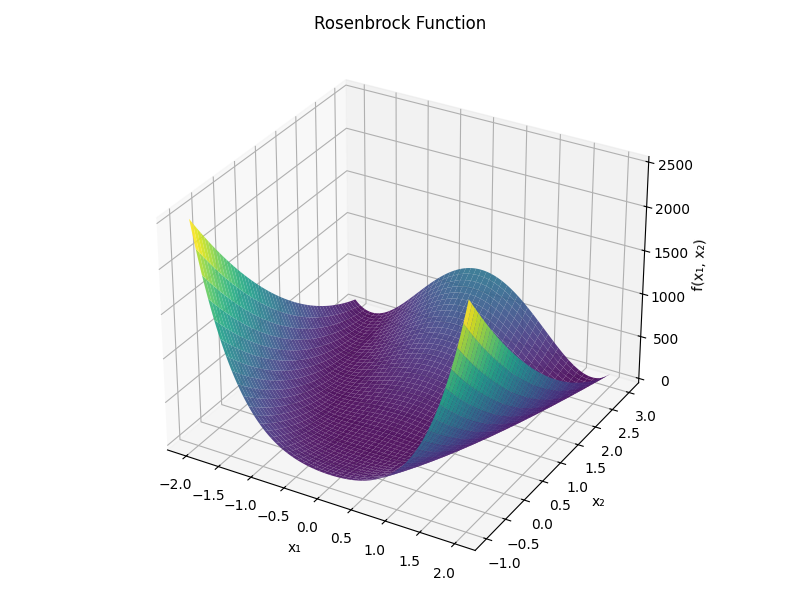
\includegraphics[width=0.7\textwidth]{../immagini/rosen3D_A.png}
		\caption{Surface plot of the Rosenbrock function over the domain $[-2, 2] \times [-1, 3]$. The function exhibits a narrow curved valley with a global minimum at $(1, 1)$, where $f(x) = 0$. This geometry makes it a standard benchmark for testing unconstrained optimization algorithms.}
		
		\label{fig:rosennewton}
	\end{figure}
	\newpage
	
	\vspace{1em}
	\textbf{Modified Newton Method} results:
	\begin{itemize}
		\item From \( x^{(0)}_A \):  
		minimum found at \( (1.000050,\;1.000083) \),  
		function value: \( 0.000000 \),  
		iterations: 6.
		\item From \( x^{(0)}_B \):  
		minimum found at \( (0.999995,\;0.999990) \),  
		function value: \( 0.000000 \),  
		iterations: 21.
	\end{itemize}
	
	\begin{figure}[htbp]
		\centering
		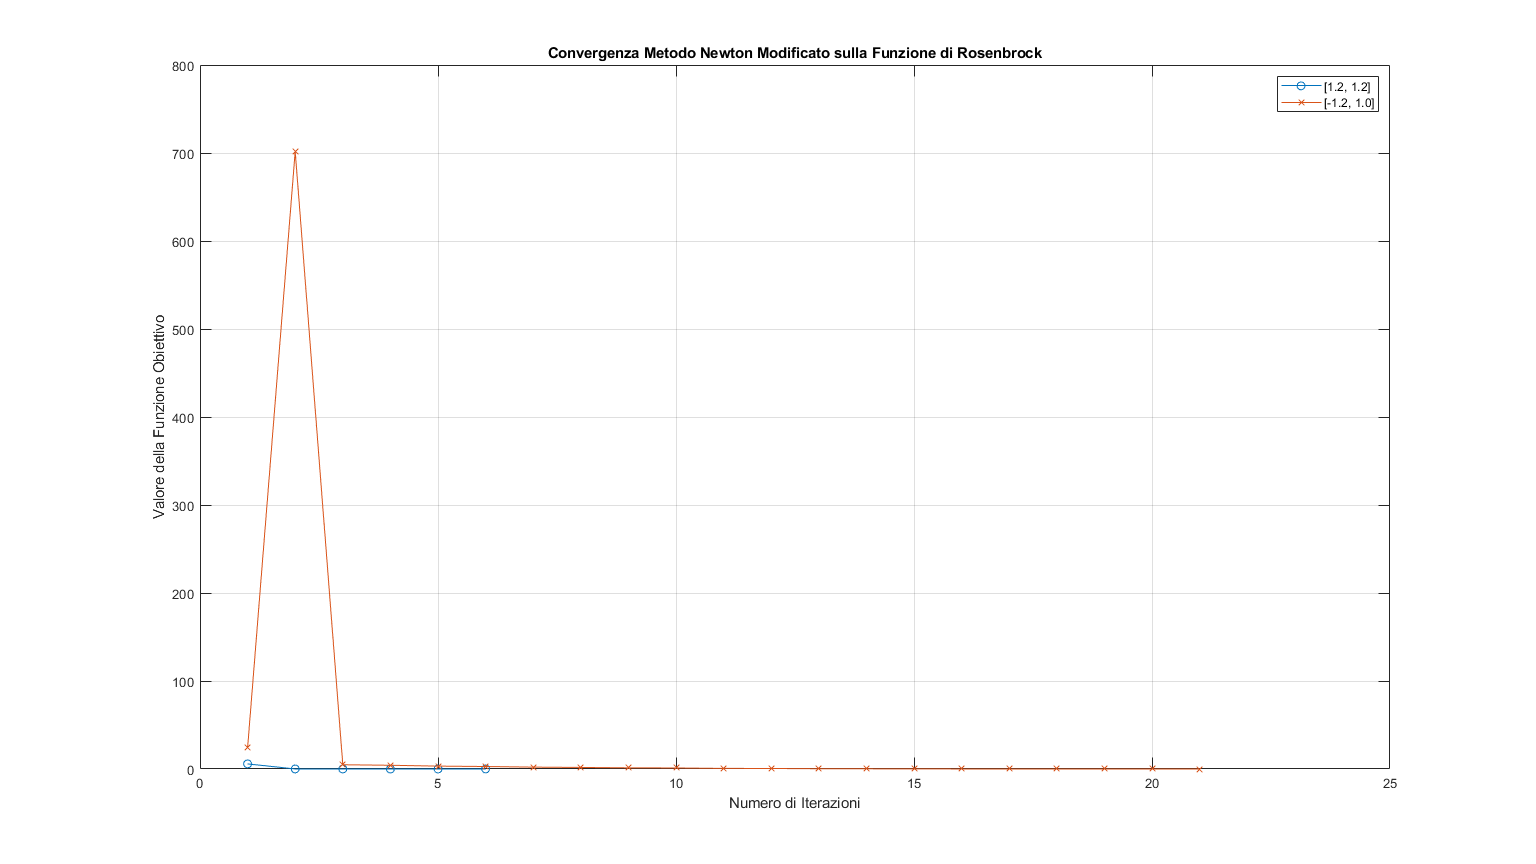
\includegraphics[width=0.7\textwidth]{../immagini/grafrosennewton.png}
		\caption{Convergence behaviour of the Modified Newton method on the Rosenbrock function starting from $x^{(0)} = [1.2, 1.2]$ and $x^{(0)} = [-1.2, 1.0]$.}
		\label{fig:rosennewton}
	\end{figure}
	
	\newpage
	\vspace{1em}
	\textbf{Nelder–Mead Method} results:
	\begin{itemize}
		\item From \( x^{(0)}_A \):  
		minimum found at \( (0.999741,\;0.999441) \),  
		function value: \( 0.000000 \),  
		iterations: 58.
		\item From \( x^{(0)}_B \):  
		minimum found at \( (1.222612,\;1.488895) \),  
		function value: \( 0.053018 \),  
		iterations: 29.
	\end{itemize}
	
	\begin{figure}[htbp]
		\centering
		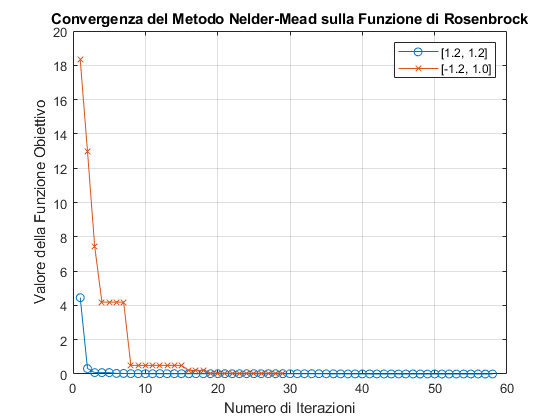
\includegraphics[width=0.7\textwidth]{../immagini/grafrosennelder.png}
		\caption{Convergence behaviour of the Nelder Mead method on the Rosenbrock function starting from $x^{(0)} = [1.2, 1.2]$ and $x^{(0)} = [-1.2, 1.0]$.}
		\label{fig:rosennewton}
	\end{figure}
	
	\vspace{1em}
	
	
	\vspace{1em}
	\textbf{Discussion.}  
	Both methods converge from \( x^{(0)}_A \), although Modified Newton reaches the solution significantly faster (6 iterations vs.\ 58). From the more challenging initial point \( x^{(0)}_B \), the Newton method again converges reliably, while Nelder–Mead gets stuck in a suboptimal region, with higher final function value and fewer iterations. This confirms the advantage of second-order information for curved valleys.
	
	 
	
	\section{Extended Rosenbrock Function}
	\subsection{Exact Gradient and Hessian}
	\subsection{Finite Differences Gradient and Hessian}
	
	\section{Generalized Broyden Tridiagonal Function}
	\subsection{Exact Gradient and Hessian}
	\subsection{Finite Differences Gradient and Hessian}
	
	\section{Banded Trigonometric Function}
	\subsection{Exact Gradient and Hessian}
	\subsection{Finite Differences Gradient and Hessian}
	
	\section{Conclusions}
	
	% -------------------------------------------------
	\appendix              % da qui in poi usa lettere (A, B…)
	% -------------------------------------------------
	\section{Code snippets}
	\subsection{Code for Method Implementations}
	\subsubsection{Modified Newton Method}
	\subsubsection{Truncated Newton Method}
	\subsection{Code for Objective Functions}
	\subsubsection{Rosenbrock Function}
	\subsubsection{Extended Rosenbrock Function}
	\subsubsection{Generalized Broyden Tridiagonal Function}
	\subsubsection{Banded Trigonometric Problem}
	\subsection{Utility Code for Running Experiments}
	
\end{document}
